\documentclass[dvipsnames, tikz]{standalone}

% better text rendering
% https://tex.stackexchange.com/questions/664/why-should-i-use-usepackaget1fontenc
\newcommand{\usefonts}
{
  \usepackage[T1]{fontenc}
  \usepackage[utf8]{inputenc}
  \usepackage{microtype}
  \usepackage[l]{plex-serif}
  \usepackage{plex-mono}
}

% helpers
\newcommand{\subfigwidth}{0.49\linewidth}

\newcommand{\code}[1]{\lstinline{#1}}

\newcommand
{\captiondesc}
[1]
{
  \centering
  \vspace{0.5em}
  \parbox{0.8\linewidth}{\footnotesize{}#1}
}

\newcommand{\dd}[1]{\ensuremath{#1}}
\newcommand{\dddd}[2]{\ensuremath{\dd{#1},\,\dd{#2}}}

\newcommand{\dms}[3]{\ensuremath{\ang{#1}\,#2'\,#3''}}
\newcommand{\dmsdms}[6]{\ensuremath{\dms{#1}{#2}{#3},\,\dms{#4}{#5}{#6}}}

\usefonts{}
\usepackage[simplified]{pgf-umlcd}

\setlength{\tabcolsep}{0.25em}
\renewcommand{\arraystretch}{1.2}

\renewcommand{\umltextcolor}{black}
\renewcommand{\umldrawcolor}{black}
\renewcommand{\umlfillcolor}{white}

\newcommand{\attributes}[1]
{
  \attribute{
    \centering
    \begin{tabular}{@{}lll@{}}
      #1
    \end{tabular}
    }
}

\begin{document}
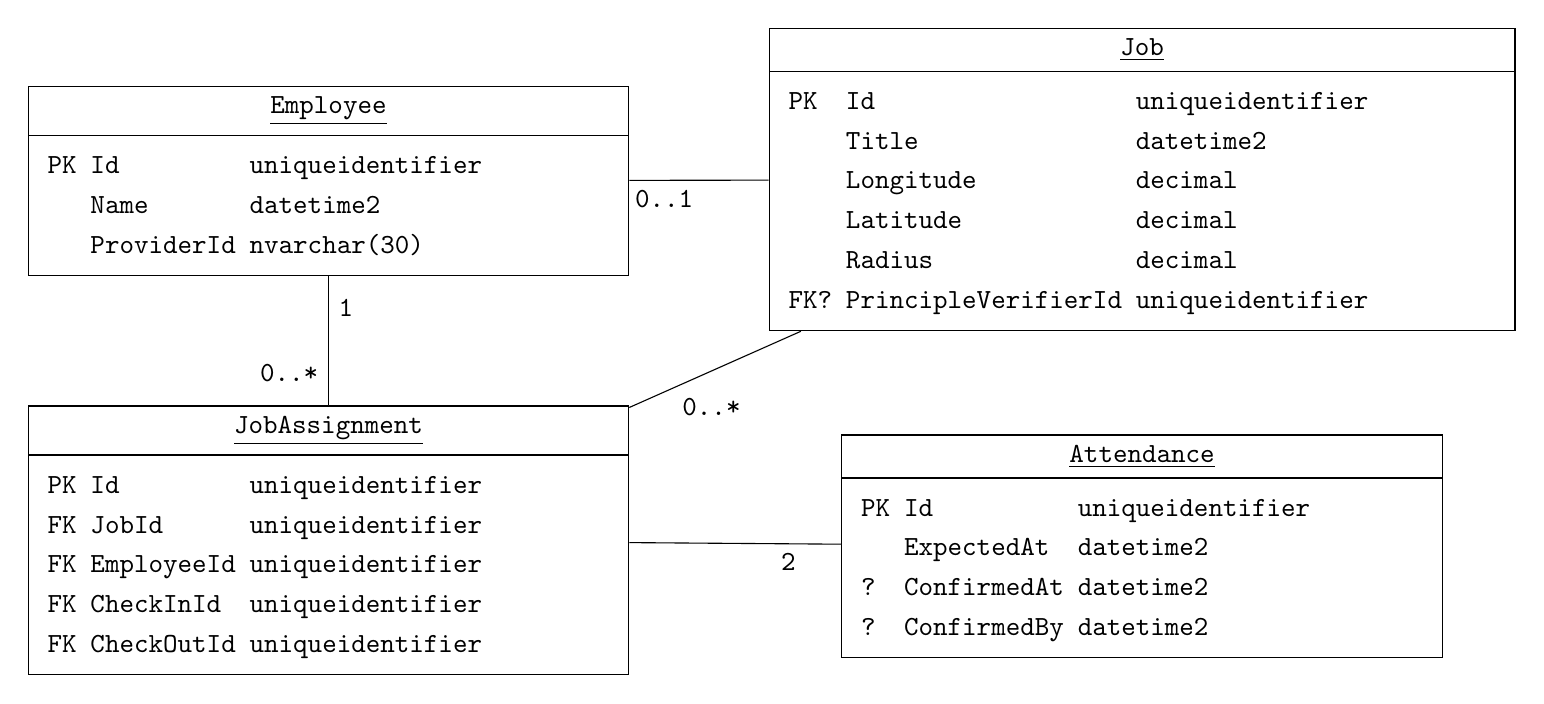
\begin{tikzpicture}
  \ttfamily

  \begin{object}[text width=20em]{Employee}{0,0}
    \attributes
    {
      PK & Id	        & uniqueidentifier \\
         & Name       & datetime2        \\
         & ProviderId & nvarchar(30)
    }
  \end{object}

  \begin{object}[text width=20em]{JobAssignment}{0,-11em}
    \attributes
    {
      PK & Id         & uniqueidentifier \\
      FK & JobId      & uniqueidentifier \\
      FK & EmployeeId & uniqueidentifier \\
      FK & CheckInId  & uniqueidentifier \\
      FK & CheckOutId & uniqueidentifier
    }
  \end{object}

  \begin{object}[text width=20em]{Attendance}{28em,-12em}
    \attributes
    {
      PK & Id          & uniqueidentifier \\
         & ExpectedAt  & datetime2        \\
      ?  & ConfirmedAt & datetime2        \\
      ?  & ConfirmedBy & datetime2
    }
  \end{object}

  \begin{object}[text width=25em]{Job}{28em,2em}
    \attributes
    {
      PK  & Id	                & uniqueidentifier \\
          & Title               & datetime2        \\
          & Longitude           & decimal          \\
          & Latitude            & decimal          \\
          & Radius              & decimal          \\
      FK? & PrincipleVerifierId & uniqueidentifier
    }
  \end{object}

  \association{Job}{}{}{Employee}{0..1}{}
  \association{Job}{}{}{JobAssignment}{0..*}{}
  \association{Employee}{1}{}{JobAssignment}{}{0..*}
  \association{Attendance}{2}{}{JobAssignment}{}{}

\end{tikzpicture}
\end{document}
